% LTeX: enabled=true

\subsection{Important Notation}

To avoid ambiguity, we introduce the following notation conventions used throughout the paper.
For any $n \in \mathbb{N}$, we write $[n] \triangleq \{1, \ldots, n\}$  and $[n]_0 \triangleq [n] \cup \{0\}$. 
We define the Boolean domain as $\mathbb{B} \triangleq \{0, 1\}$ and
three value domain $\mathbb{T} \triangleq \{0, 1, \bot\}$.


\subsection{Background overview}


\subsubsection{Counting Complexity and Combinatorial Interpretations}

Counting complexity looks into complexity of counting solutions using notions
such as $\textbf{\#P}$.
$\textbf{\#P}$ was created by \cite{valiant_ComplexityComputingPermanent_1979},
to demonstrate the difficulty of counting the number of solutions to a problem,
even they are polynomially verifiable.

\begin{definitionbox}{$\textsc{\#P}$ Complexity Clas \cite{valiant_ComplexityComputingPermanent_1979}}{sharpp-class}
    $\textbf{\#P}$ is a class of functions $f: \{0,1\}^* \to \mathbb{N}$
    such that: there
    exists a polynomial-time deterministic TM $M$, and
    $p : \mathbb{N} \to \mathbb{N}$ such that $p \in n^{O(1)}$, we have:
    $$
    f(w) = \Big|\Big\{v \in \{0,1\}^{p(|w|)} \mid M(w, v) =1 \Big\}\Big|
    $$
\end{definitionbox}


As we can see, $\textbf{\#P}$ allows us to define a set of objects,
whose cardinality equals $f(w)$. The reason for choosing
$\textbf{\#P}$ to define combinatorial interpretations is \cite{ikenmeyer_PositivitySymmetricGroup_2024}: 

\begin{enumerate}
    \item By polynomially bounding words, we avoid cases such as: $f(w) = |\{1, \hdots, f(w)\}|$.
    \item Current framework allows us to work with $f(\cdot)$, whose direct computation can be computationally hard.
\end{enumerate}


The current framework was used in several papers such as
\cite{ikenmeyer_WhatWhatNot_2022} and \cite{ikenmeyer_PositivitySymmetricGroup_2024}
where they were able to use tools from complexity theory to show that
many structures do or do not have a combinatorial interpretation.
For the purposes of the current project, we are focusing on \cite{ikenmeyer_WhatWhatNot_2022},
and $\textsc{TFNP}$ problems.
Lastly we introduce the idea of correlating two counting problems with the help of
\textit{parsimonious reductions} \ref{def:pars-reduction}.


\begin{definitionbox}{Parsimonious reductions}{pars-reduction}
    Let $R, R'$ be search problems and let $f$ be a reduction of
    $S_R = \{x \mid R(x) \neq \emptyset \}$ to $S_{R'} = \{x \mid R'(x) \neq \emptyset \}$.
    We say $f$ is \textbf{parsimonious} if:
    $$
    \forall x \in S_R : |R(x)| = |R'(f(x))|
    $$ 
\end{definitionbox}

Below we are introducing a variant of parimonious reductions that allows
for one-to-many reductions. 
\begin{definitionbox}{Poly-Function Bounded Parsimonious Reductions}{func-pars}
    Given two counting problems $A, B : \{0,1\}* \to \mathbb{N}$
    and a function $f : {0,1}^{*} \to \mathbb{N}$ such that $f \in n^{O(1)}$, we
    say that:
    $$
    A \subseteq^f B
    $$
    If for input $w \in \{0,1\}^*$, if $a$ represent the number of solutions
    for problem $A$ and $b$ the number of solutions for problem $B$, we have:
    $$
    a \leq b \leq f(|w|) \cdot a
    $$
    If $\forall x : f(x) = c$ for $c \in \mathbb{N}$ then we will just say 
    $$
    A \subseteq^c B
    $$
\end{definitionbox}

\subsubsection{Total Search Problems and PPAD}
We give a brief overview of \textbf{TFNP} and \textbf{PPAD}.


\begin{definitionbox}{Search Problems and Total Search Problems}{search-problems}
    \textbf{Search problems} can be defined as relations $R \subseteq \{0,1\}^* \times \{0,1\}^*$,
    where given $x \in \{0,1\}^*$, we want to find $y \in \{0,1\}^*$  such that $x Ry$.

    \textbf{Total Search problems} are search problems such that:
    $$
    \forall x \in \{0,1\}^*, \exists y \in \{0,1\}^* : xRy
    $$
\end{definitionbox}


\begin{definitionbox}{$\scn{FNP}$ and $\scn{TFNP}$}{fnp-tfnp}
    \textbf{FNP} are \textit{search problems} such that there exists poly-time TM $M: \{0,1\}^* \to \{0,1\}$
    and a poly function $p : \mathbb{N} \to \mathbb{N}$ such that:
    $$
    \forall x \in \{0,1\}^*, y \in \{0,1\}^{p(|x|)}: xRy \iff M(x,y) = 1
    $$
    Lastly $\textbf{TFNP} = \{L \in \textbf{FNP} \mid L \text{ is total}\}$
\end{definitionbox}

%
% \begin{definitionbox}{Levin Reductions}{levin-red}
%     Given a pair of search problems $R_A, R_B$, a pair of
%     computable time functions $(f,g)$ is called a Levin reduction from $R_A \to R_B$
%     \begin{gather*}
%         S_R \triangleq \{x \mid \exists y : xRy  \}\\
%         R(x) \triangleq \{y \mid x Ry \} \\
%         \forall x \in S_{R_A}, y_b \in R(f(x)):  (x , g(x, y_b)) \in R_A
%     \end{gather*}
% \end{definitionbox}


Our current work focuses on a specific subclass of $\textbf{TFNP}$ problems
which is defined as follows:

\begin{definitionbox}{\textit{EndOfLine} problem \cite{papadimitriou_ComplexityParityArgument_1994}}{eol-ppad}
    Given circuits $S, P \in \{0,1\}^n \to \{0,1\}^n$ such that $S,P \in n^{O(1)}$
    we define a directed graph $G = (V,E)$, such that $V= \{0,1\}^n$ and $E$ defined as:
    $$
    E = \{(x,y) \in V^2: S(x) = y \wedge P(y) = x\}
    $$
    We define source or sinks $\forall v \in V: \textit{deg}(v) = (0,1)$ or
    $\textit{deg}(v) = (1,0)$, respectively. 
    We also syntactially ensure that the $0^n$ node is always a source, meaning
    $S(P(0^n) \neq 0 \wedge P(S(0^n)) = 0^n$.
    A node $v \in V$ is a solution if and only if $\textit{deg}(v)$ is either
    $(0,1)$  or $(1,0)$.
\end{definitionbox}


\begin{figure}[h!]
    \centering
    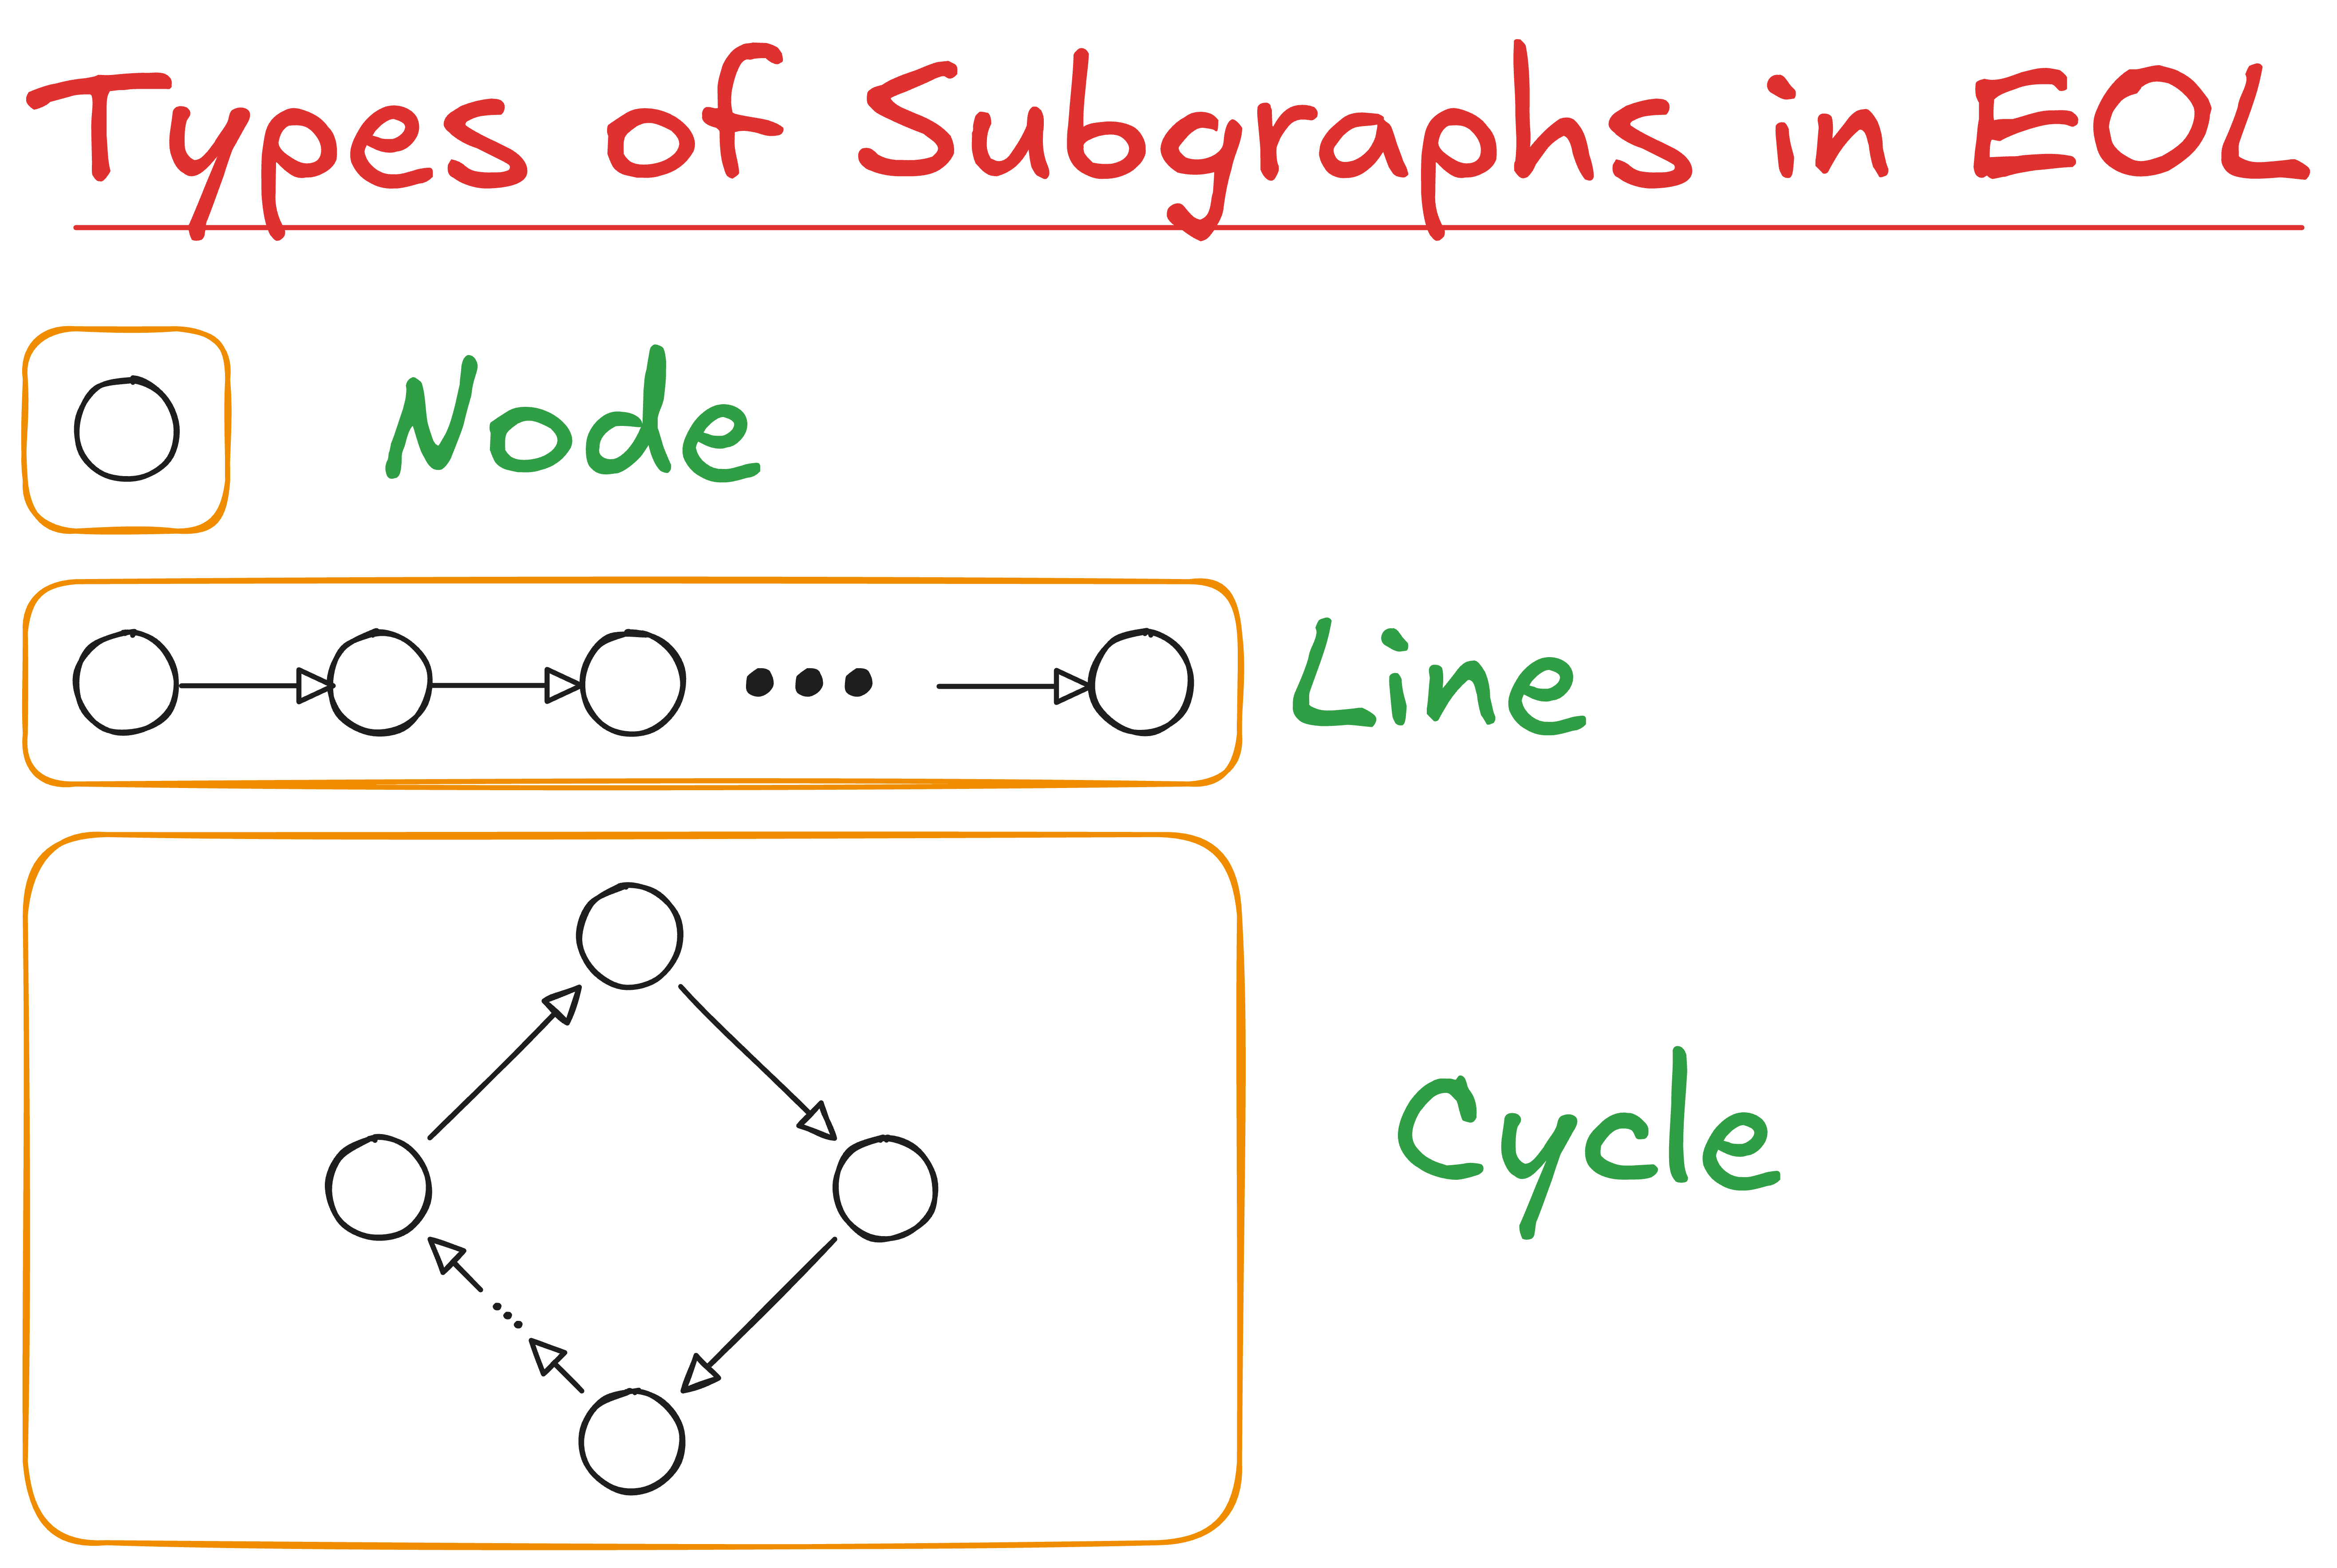
\includegraphics[width=0.3\textwidth]{assets/eol-subgraphs.png}
    \caption{Types of subgraphs in \textsc{EndOfLine}}\label{fig:eol-subgraphs}
\end{figure}


An illustrative example of an instance can be seen in the figure \ref{fig:eol-subgraphs}. 
Using the \textsc{EndOfLine} problem, we define the
\textsc{PPAD} complexity class \ref{def:ppad-complexity-class}


\begin{definitionbox}{\textsc{PPAD} complexity class \cite{papadimitriou_ComplexityParityArgument_1994}}{ppad-complexity-class}
    \textsc{PPAD} is defined as the set of search problems that
    are reducible to the \scn{EndOfLine} problem \ref{def:eol-ppad}.
\end{definitionbox}

\textbf{PPAD} has been created by Papadimitriou \cite{papadimitriou_ComplexityParityArgument_1994}
to demonstrate a subset of problems in \textbf{NP} that are guaranteed to have
a solution but can be very difficult to find. In the next section
we will introduce the relevant of \textsc{PPAD} problems.

\paragraph{The PureCircuit problem}
\label{par:pure-circ-def}

The  \textsc{PureCircuit} was created by Deligkas et al. \cite{deligkas_PureCircuitTightInapproximability_2024}
to demonstrate the hardness of approximating \textsc{PPAD} problems.
it uses kleene-logic based circuits and with continuity of arguments, they demonstrated \textsc{PPAD-completeness}.

\begin{definitionbox}{\textsc{PureCiruit} Problem Definition \cite{deligkas_PureCircuitTightInapproximability_2024}}{purecircuit-def}
An instance of \textit{PureCircuit} is given by vertex set $V= [n]$ and gate set $G$ such that
$\forall g \in G: g=(T,u,v,w)$ where $u,v,w \in V$ and $T \in \{\text{NOR}, \text{Purify}\}$.
Each gate is interpreted as:
\begin{enumerate}
    \item \textit{NOR}: Takes as input $u,v$ and outputs $w$
    \item \textit{Purify}: Takes as input $u$ and outputs $v,w$
\end{enumerate}
And each vertex is ensured to have $\text{in-deg}(v) \leq 1$.
A solution to input instance $(V,G)$ is denoted as an assignment $\mathbf{x} : V \to \{0, \bot, 1\}$
such that for all nodes we have:
\begin{enumerate}
    \item if $v$ is the output of a $(\textit{NOR}, u,v,w)$ gate:
       \begin{gather*}
            \mathbf{x}[u] = \mathbf{x}[v] = 0 \implies \mathbf{x}[w] = 1\\
            (\mathbf{x}[u] =1 \vee \mathbf{x}[v] =1) \implies \mathbf{x}[w] = 0 \\
            \text{otherwise} \implies \bot
        \end{gather*}

    \item \textit{Purify}: 
       \begin{gather*}
           \forall b \in \{0,1\}: \mathbf{x}[u] = b \implies \mathbf{x}[v] = b \wedge \mathbf{x}[w] =  b\\
           \mathbf{x}[u] = \bot \implies \{\mathbf{x}[v] \cup \mathbf{x}[w] \} \cap \{0,1\} \neq \emptyset
        \end{gather*}
\end{enumerate}
\end{definitionbox}

The definition of \textsc{PureCircuit} that we will be using for the standard set of gates
$\{\wedge, \vee, \neg\}$, is based Kleene's three-valued strong logic of indeterminancy
which extends the traditional $\mathbb{B}$ logic \cite{kleene_IntroductionMetamathematics_2009}.
Their behaviour can be described in the tables shown in \ref{tab:three-val-logic}
In addition to that, we will make use of the \textit{Copy} gate which we can define as $\textit{Copy}(x) = \neg (\neg x)$.
This allows our circuits to be robust and easier to work with.

\begin{table}[h!]
    \centering
    \subfloat[\texttt{not} gate]{
    \begin{tabular}{c|c}
\texttt{not} & \textbf{} \\
\hline
0 & 1 \\
$\bot$ & $\bot$ \\
1 & 0 \\
\end{tabular}
}
\subfloat[\texttt{and} gate]{
\begin{tabular}{c|ccc}
\texttt{and} & 0 & $\bot$ & 1 \\
\hline
0    & 0 & 0 & 0 \\
$\bot$ & 0 & $\bot$ & $\bot$ \\
1    & 0 & $\bot$ & 1 \\
\end{tabular}
} \quad
\subfloat[\texttt{or} gate]{
\begin{tabular}{c|ccc}
\texttt{or} & 0 & $\bot$ & 1 \\
\hline
0    & 0     & $\bot$ & 1 \\
$\bot$ & $\bot$  & $\bot$ & 1 \\
1    & 1 & 1 & 1 \\
\end{tabular}
}

    \caption{Three-valued logic \cite{kleene_IntroductionMetamathematics_2009}}\label{tab:three-val-logic}
\end{table}




For the \textit{Purify} gate,
Deligkas et al. showed that the only solutions that are essential for \textit{Purify}
are $\{(0,\bot), (\bot,1), (0,1)\}$ with the help of continuity arguments \cite{deligkas_PureCircuitTightInapproximability_2024}.
Adding more solutions does not change the complexity as he showed in the original variant of the problem.
We acknowledge that the solution set will be different from the original one but,
one can observe that  $\textsc{\#PureCircuit-simplified} \subseteq \textsc{\#PureCircuit}$,
and therefore any proposition or argument of the sort:
$\textsc{\#A} \subseteq \textsc{\#PureCircuit-simplified} \implies \textsc{\#A} \subseteq \textsc{\#PureCircuit}$.
For the purposes of the report, any solution change will be made explicit
and we will refer to all such simplified variants as $\textsc{\#PureCircuit}$ to avoid
confusion. 



\begin{definitionbox}{\textsc{SourceOrExcess} problem}{source-or-excess}
    We define as $\textit{SourceOrExcess}(k,1)$ for $k \in \mathbb{N}_{\geq 2}$
    the search problem as such: Given a poly-sized successor circuit $S : \{0,1\}^n$
    and a set of predecssor poly-sized circuits $\{P_i\}_{i \in [k]}$, we define
    the graph $G = (V,E)$ such that, $V = \{0,1\}^n$ and $E$ as:
    $$
    \forall x, y \in V: (x,y) \in E \iff (S(x) = y) \wedge \bigvee_{i \in [k]} P_i(y) = x
    $$
    We ensure that $0^n$ is as sink, meaning $\text{deg}(0^n) = (0,1)$.
    A valid solution is a vertex $v$ such that $\textit{in-deg}(v) \neq \textit{out-deg}(v)$
\end{definitionbox}

\paragraph{Sperner problems}

Below we will refer to the notion of Sperner problems which involve
the idea of using the topology of a problem and a colouring scheme to ensure
that a substructure is panchromatic. There two variants of colouring scheme
that are used: one of them will be referred to as the \textbf{linear} colouring
where for dimension $d$, assign $d+1$ distinct colours to each point \cite{daskalakis_ComplexityComputingNash_2006, chen_Complexity2DDiscrete_2009}.
Below we will refer to \textbf{bipolar} colouring, which has been used grid-like topologies of the Sperner property
\cite{chen_SettlingComplexityComputing_2009, deligkas_PureCircuitTightInapproximability_2024, daskalakis_ComplexityConstrainedMinmax_2021}.
It has to be noted that these are not their official names, but we have decided
to use this naming scheme for clarity.



\begin{definitionbox}{Bipolar colouring}{bipolar-colouring}
    Given dimension $d$, we refer to the bipolar colouring $C$ of a point $v \in S^d$
    where $S$ is some arbitrary set in $d$ dimensionality the following:
    $$
    \forall j \in [d]: [C(v)]_j \in \{-1,1\}
    $$
    Essentially a point is a associate with a $d$ dimensionaly binary vector.
    We say that a set of points $A \subseteq S^d$ \textbf{cover all the labels} if:
    $$
        \forall i \in [d], \ell \in \{-1, +1\}, \exists x \in A: [\lambda(x)]_{i} = \ell
    $$
\end{definitionbox}



\begin{definitionbox}{\textsc{StrongSperner} problem}{strong-sperner}
    \textbf{Input}: A boolean circuit that computes a bipolar labelling $\lambda: [M]^N \to \{-1, 1\}^N$ \ref{def:bipolar-colouring}
    satisfying the following boundary conditions $\forall i \in [N]$:
    \begin{itemize}
        \item if $x_i = 1 \implies [\lambda(x)]_i = +1$
        \item if $x_i = M \implies [\lambda(x)]_i = -1$
    \end{itemize}
    \textbf{Output}: A set of points $\{x^{(i)}\}_{i \in [N]} \subseteq [M]^{[N]}$, such that:
    \begin{itemize}
        \item \textit{Closessness condition}: $\forall i,j \in [N]: \|x^{(i)} - x^{(j)}\|_{\infty} \leq 1$
        \item \textit{Covers all labels} as defined in \ref{def:bipolar-colouring}
    \end{itemize}
\end{definitionbox}

The above is a generalised variant of the tradtional Sperner problem to
a grid of dimensions $N$ and width of $M$. 
Throughout literature the same variants of the problem or specifications
have been defined using sperner or discrete brouwer \cite{chen_SettlingComplexityComputing_2009, chen_Complexity2DDiscrete_2009, daskalakis_ComplexityComputingNash_2006, deligkas_PureCircuitTightInapproximability_2024}.
For the sake of clarity, we will stick to $\textsc{StrongSperner}$.

\begin{definitionbox}{$\scn{nD-StrongSperner}$ problem}{nd-strong-sperner}
    \textbf{Input}: A tuple $(\lambda,0^k)$ of a $\scn{StrongSperner}$ instance but for only $n$ dimensions, such that
    $\lambda : (\{0,1\}^k)^n \to \{-1, +1\}^n$.\\
    \textbf{Output}: A point $\alpha = (a_1, \hdots, a_n) \in A^n$, where $A=\{0,1\}^k \setminus \{1^k\}$ such that:
    $$
    \{\alpha + x \mid x \in \{0,1\}^n\} \text{ cover all the labels \ref{def:bipolar-colouring}}
    $$
    We use $A$ to avoid edge cases. We assume dimensionality $n \geq 2$.
\end{definitionbox}

Chen et al. \cite{chen_SettlingComplexityComputing_2009} demonstrated 
that all $\textsc{nD-StrongSperner}$ are $\textsc{PPAD-complete}$.
We mainly use this to show counting arguments with respect to the
\textsc{EndOfLine} as people have indicated a parsimonious reduction
between $\textsc{2D-StrongSperner}$ 
and $\textsc{3D-StrongSperner}$ to the EndOfLine problem but 
with \textit{linear} colouring. The authors of these papers
use these problems indifferently when talking about the reductions
and therefore we can assume that either colouring will create a correct reduction.

\paragraph{Other PPAD problems} 

We will define several problems in \textsc{PPAD} that are related with our project
and demonstrate the counting complexity of \textsc{PureCircuit}.

\begin{definitionbox}{\textsc{SourceOrExcess} problem}{source-or-excess}
    We define as $\textit{SourceOrExcess}(k,1)$ for $k \in \mathbb{N}_{\geq 2}$
    the search problem as such: Given a poly-sized successor circuit $S : \{0,1\}^n$
    and a set of predecssor poly-sized circuits $\{P_i\}_{i \in [k]}$, we define
    the graph $G = (V,E)$ such that, $V = \{0,1\}^n$ and $E$ as:
    $$
    \forall x, y \in V: (x,y) \in E \iff (S(x) = y) \wedge \bigvee_{i \in [k]} P_i(y) = x
    $$
    We ensure that $0^n$ is as sink, meaning $\text{deg}(0^n) = (0,1)$.
    A valid solution is a vertex $v$ such that $\textit{in-deg}(v) \neq \textit{out-deg}(v)$
\end{definitionbox}

Lastly we will introduce \textsc{Tarski} \ref{def:tarski-ppad}, which is a problem in $\textsc{PLS} \cap \textsc{PPAD}$
where $\textsc{PLS}$ is a class of problems based on the idea of local search \cite{johnson_HowEasyLocal_1988}
and uses the Knaster-Tarski fixed point theorem \ref{thm:knaster-tarski}. We will use this problem in later
sections to connect Kleene algebra with \textsc{PPAD}.


\begin{definitionbox}{Monotone functions}{mono-func}
    Given two posets $(L_1, \preceq_{L_1})$ and $(L_2, \preceq_{L_2})$, a function
    $f: L_1 \to L_2$ is \textbf{monotone} if and only if:
    $$
    \forall x,y \in L_1: x \preceq_{L_1} y \implies f(x) \preceq_{L_2} f(y)
    $$
\end{definitionbox}
    

\begin{theorembox}{Knaster Tarski Fixed point theorem\cite{bronislaw_TheoremeFunctionsDensembles_1928, fearnley_FasterAlgorithmFinding_2022}}{knaster-tarski}
    Given a lattice $(L, \wedge, \vee)$ and a \textit{monotone} $f: L \to L$ \ref{def:mono-func}
    $$
    \exists c \in L: f(c) = c
    $$
\end{theorembox}

Using the Tarski theorem, Fearnley et al. \cite{fearnley_FasterAlgorithmFinding_2022}
created a \textsc{TFNP} variant of the problem which finds fixed points or 
identifies points that break the monotone argument. We will be using Tarski 
with Kleene logic to connect the two.
% \begin{definitionbox}{$\scn{Tarski}$ problem definition \cite{fearnley_FasterAlgorithmFinding_2022}}{tarski-ppad}
%     Given a lattice $(L, \wedge, \vee)$, and a \textit{monotone} function $f : L \to L$ 
%     we define solutions to the problem as:
%     \begin{enumerate}
%         \item Find $x \in L: f(x) = x$
%         \item Find $x,y \in L$ such that $x \preceq y$ and $f(x) \not\preceq f(y)$
%     \end{enumerate}
%     We assume that $f$ is described by circuit.
% \end{definitionbox}
%
\paragraph{Counting complexity of PPAD}

The current project looks on the counting complexity of such problems as despite two problems
being \textsc{PPAD-complete}, Ikenmeyer et al. \cite{pak_WhatCombinatorialInterpretation_2022} has showed examples where
their counting difficulty can differ vastly as it can be seen in the figure \ref{fig:ppad-count-hier}.

\begin{figure}[h!]
    \centering
    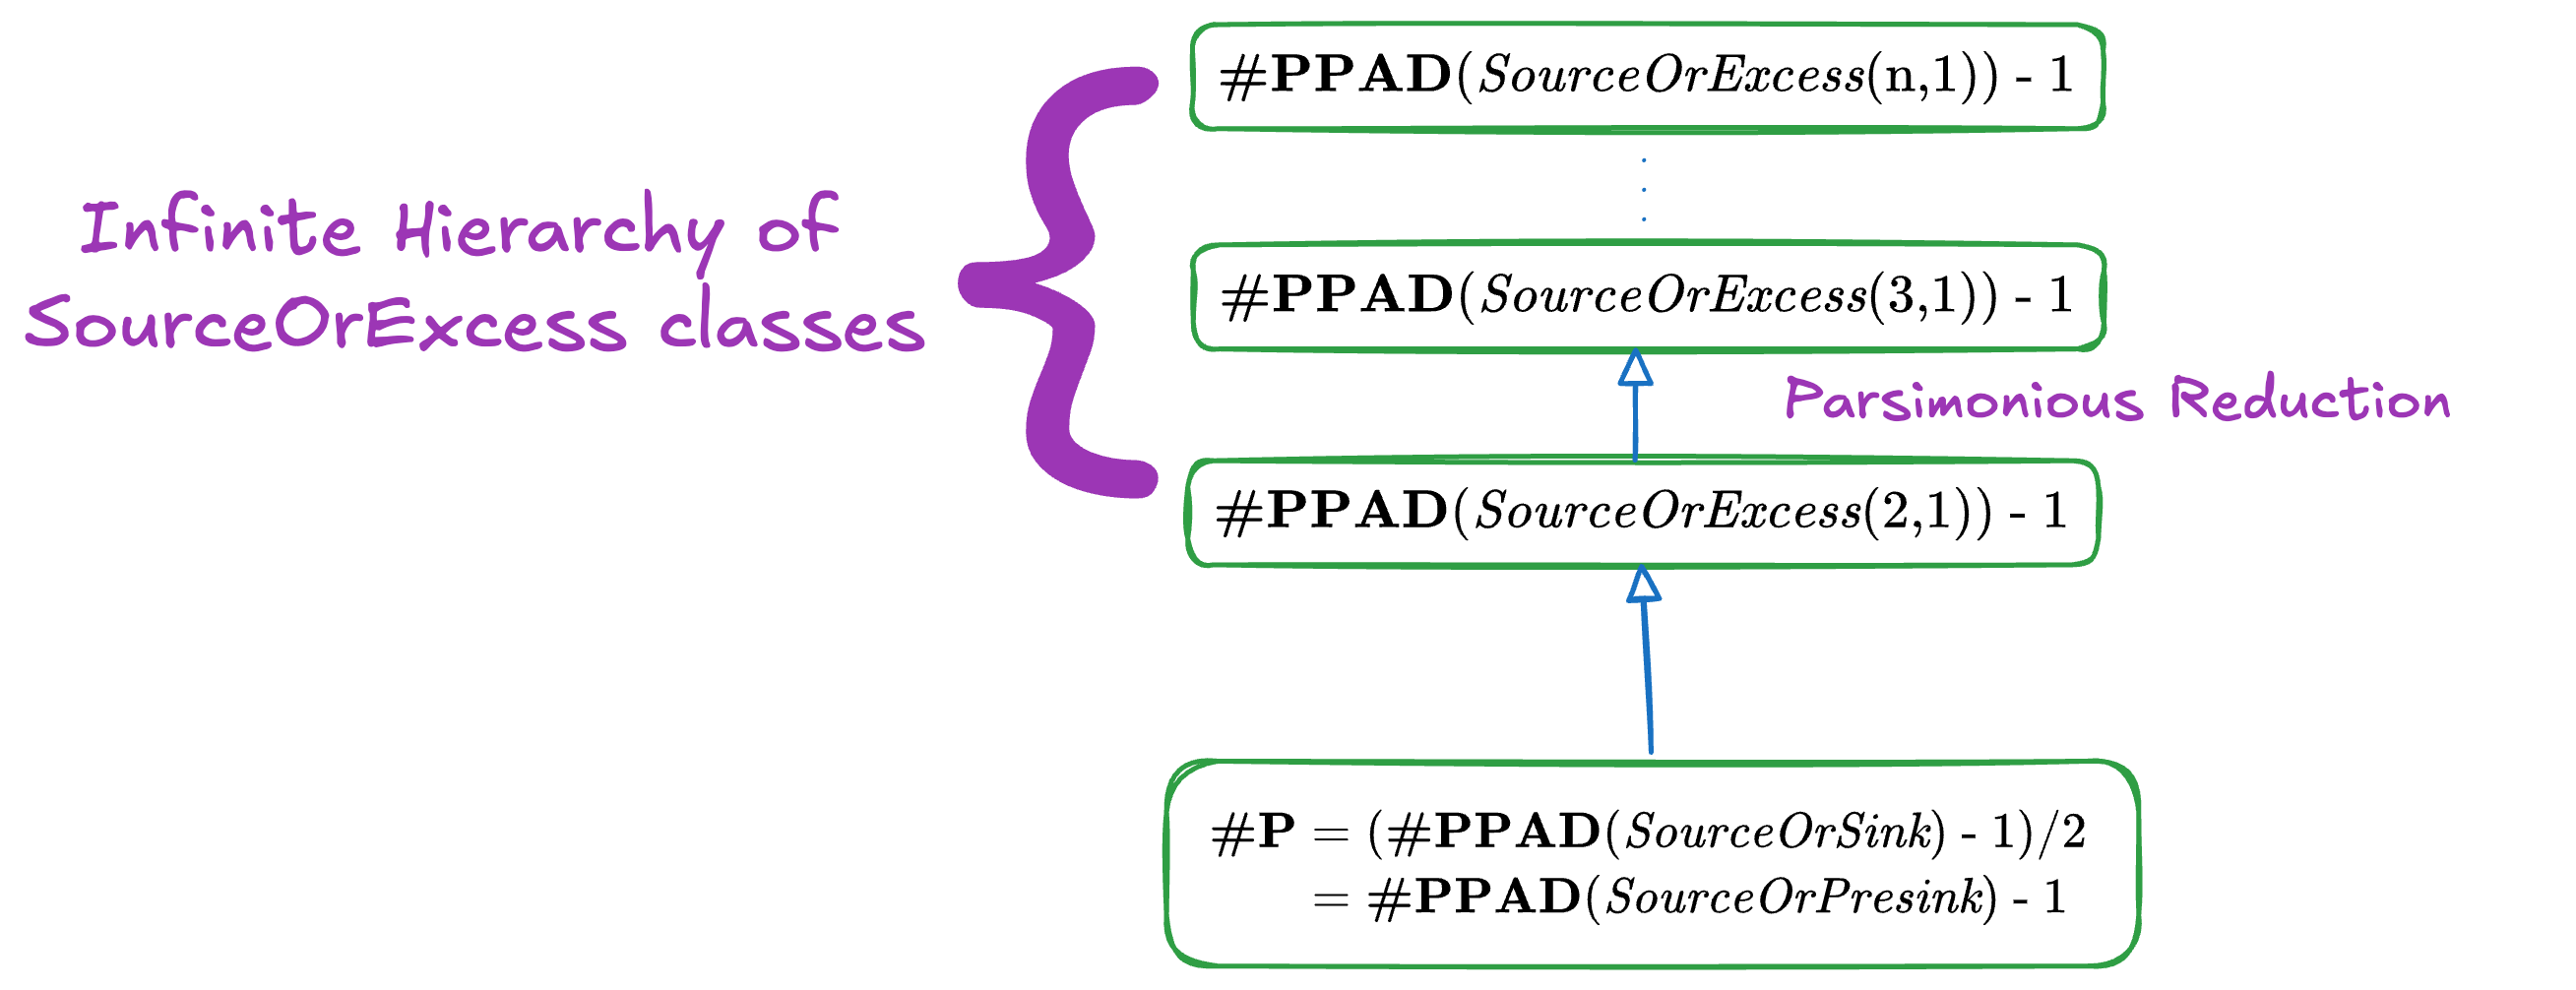
\includegraphics[width=0.5\textwidth]{assets/chart-plot.png}
    \caption{Hierarchy graph between \textsc{\#PPAD} problems. Figure from \cite{ikenmeyer_WhatWhatNot_2022}}\label{fig:ppad-count-hier}
\end{figure}


\subsubsection{Kleene Logic and Hazard-Free Circuits}

Kleene logic uses the boolean system with an additional \textit{unstable} value \cite{kleene_IntroductionMetamathematics_2009}. 
Study of Kleene logic aided in
the development of robust physical systems \cite{friedrichs_MetastabilityContainingCircuits_2018}, as well as
giving definitions to \textit{Alternative Turing mahcines} \cite{kozen_TheoryComputation_2006}, and
showing correlations complexity of monotone circuits sizes
\cite{eichelberger_HazardDetectionCombinational_1965, ikenmeyer_ComplexityHazardfreeCircuits_2019,ikenmeyer_KarchmerWigdersonGamesHazardfree_2022,  bund_SmallHazardFreeTransducers_2025}. 

Our current report will focus on specific concepts with Kleene logic as \textsc{PureCircuit} instances
use the underlying logic directly. Below we introduce important concepts \cite{mukaidono_BternaryLogicFunction_1972}.

\begin{definitionbox}{Kleene value ordering \cite{mukaidono_BternaryLogicFunction_1972}}{kleene-order}
    The instability ordering for $\leq^u$ is defined as: $\bot \leq^u 0,1$. The $n$-dimensional
    extension of the ordering is:
    $$
    \forall x,y \in \mathbb{T}^n: x \leq^u y \implies \forall j \in [n]: (x_j \in \mathbb{B} \implies x_i = y_i)
    $$
\end{definitionbox}


\begin{definitionbox}{Kleene Resolutions \cite{mukaidono_BternaryLogicFunction_1972, ikenmeyer_ComplexityHazardfreeCircuits_2019}}{kleene-res}
    Given $x \in \mathbb{T}^n$, we define the \textit{resolutions} of $x$, using the following notation:
    $$
    \scn{Res}(x) \triangleq \big\{ y \in \mathbb{B}^n \mid x \leq^u y  \big\}
    $$
\end{definitionbox}

Detecting hazards is a concept that is analysed heavily when talking about Kleene logic.
The idea is ensuring robustness of our circuits, meaning if all resolutions of $x \in \mathbb{T}^n$
give the same value, then we should expect circuit to behave the same way \ref{def:hf-def}.
An example of hazard values can be seen in the figure \ref{fig:hazard-example}.

\begin{definitionbox}{Hazard \cite{ikenmeyer_ComplexityHazardfreeCircuits_2019, eichelberger_HazardDetectionCombinational_1965}}{hf-def}
    A \textit{circuit} $C$, on $n$ inputs has \textbf{hazard} at $x \in \mathbb{T}^n \iff C(x) = \bot$
    and $\exists b \in \mathbb{B}, \forall r \in \scn{Res}(x): C(r) = b$. If such value does not exists
    then we say that $C$ is hazard-free.
\end{definitionbox}

\begin{figure}[h!]
    \centering
    \subfloat[Multiplexer with hazard at $(1,1,\bot)$]{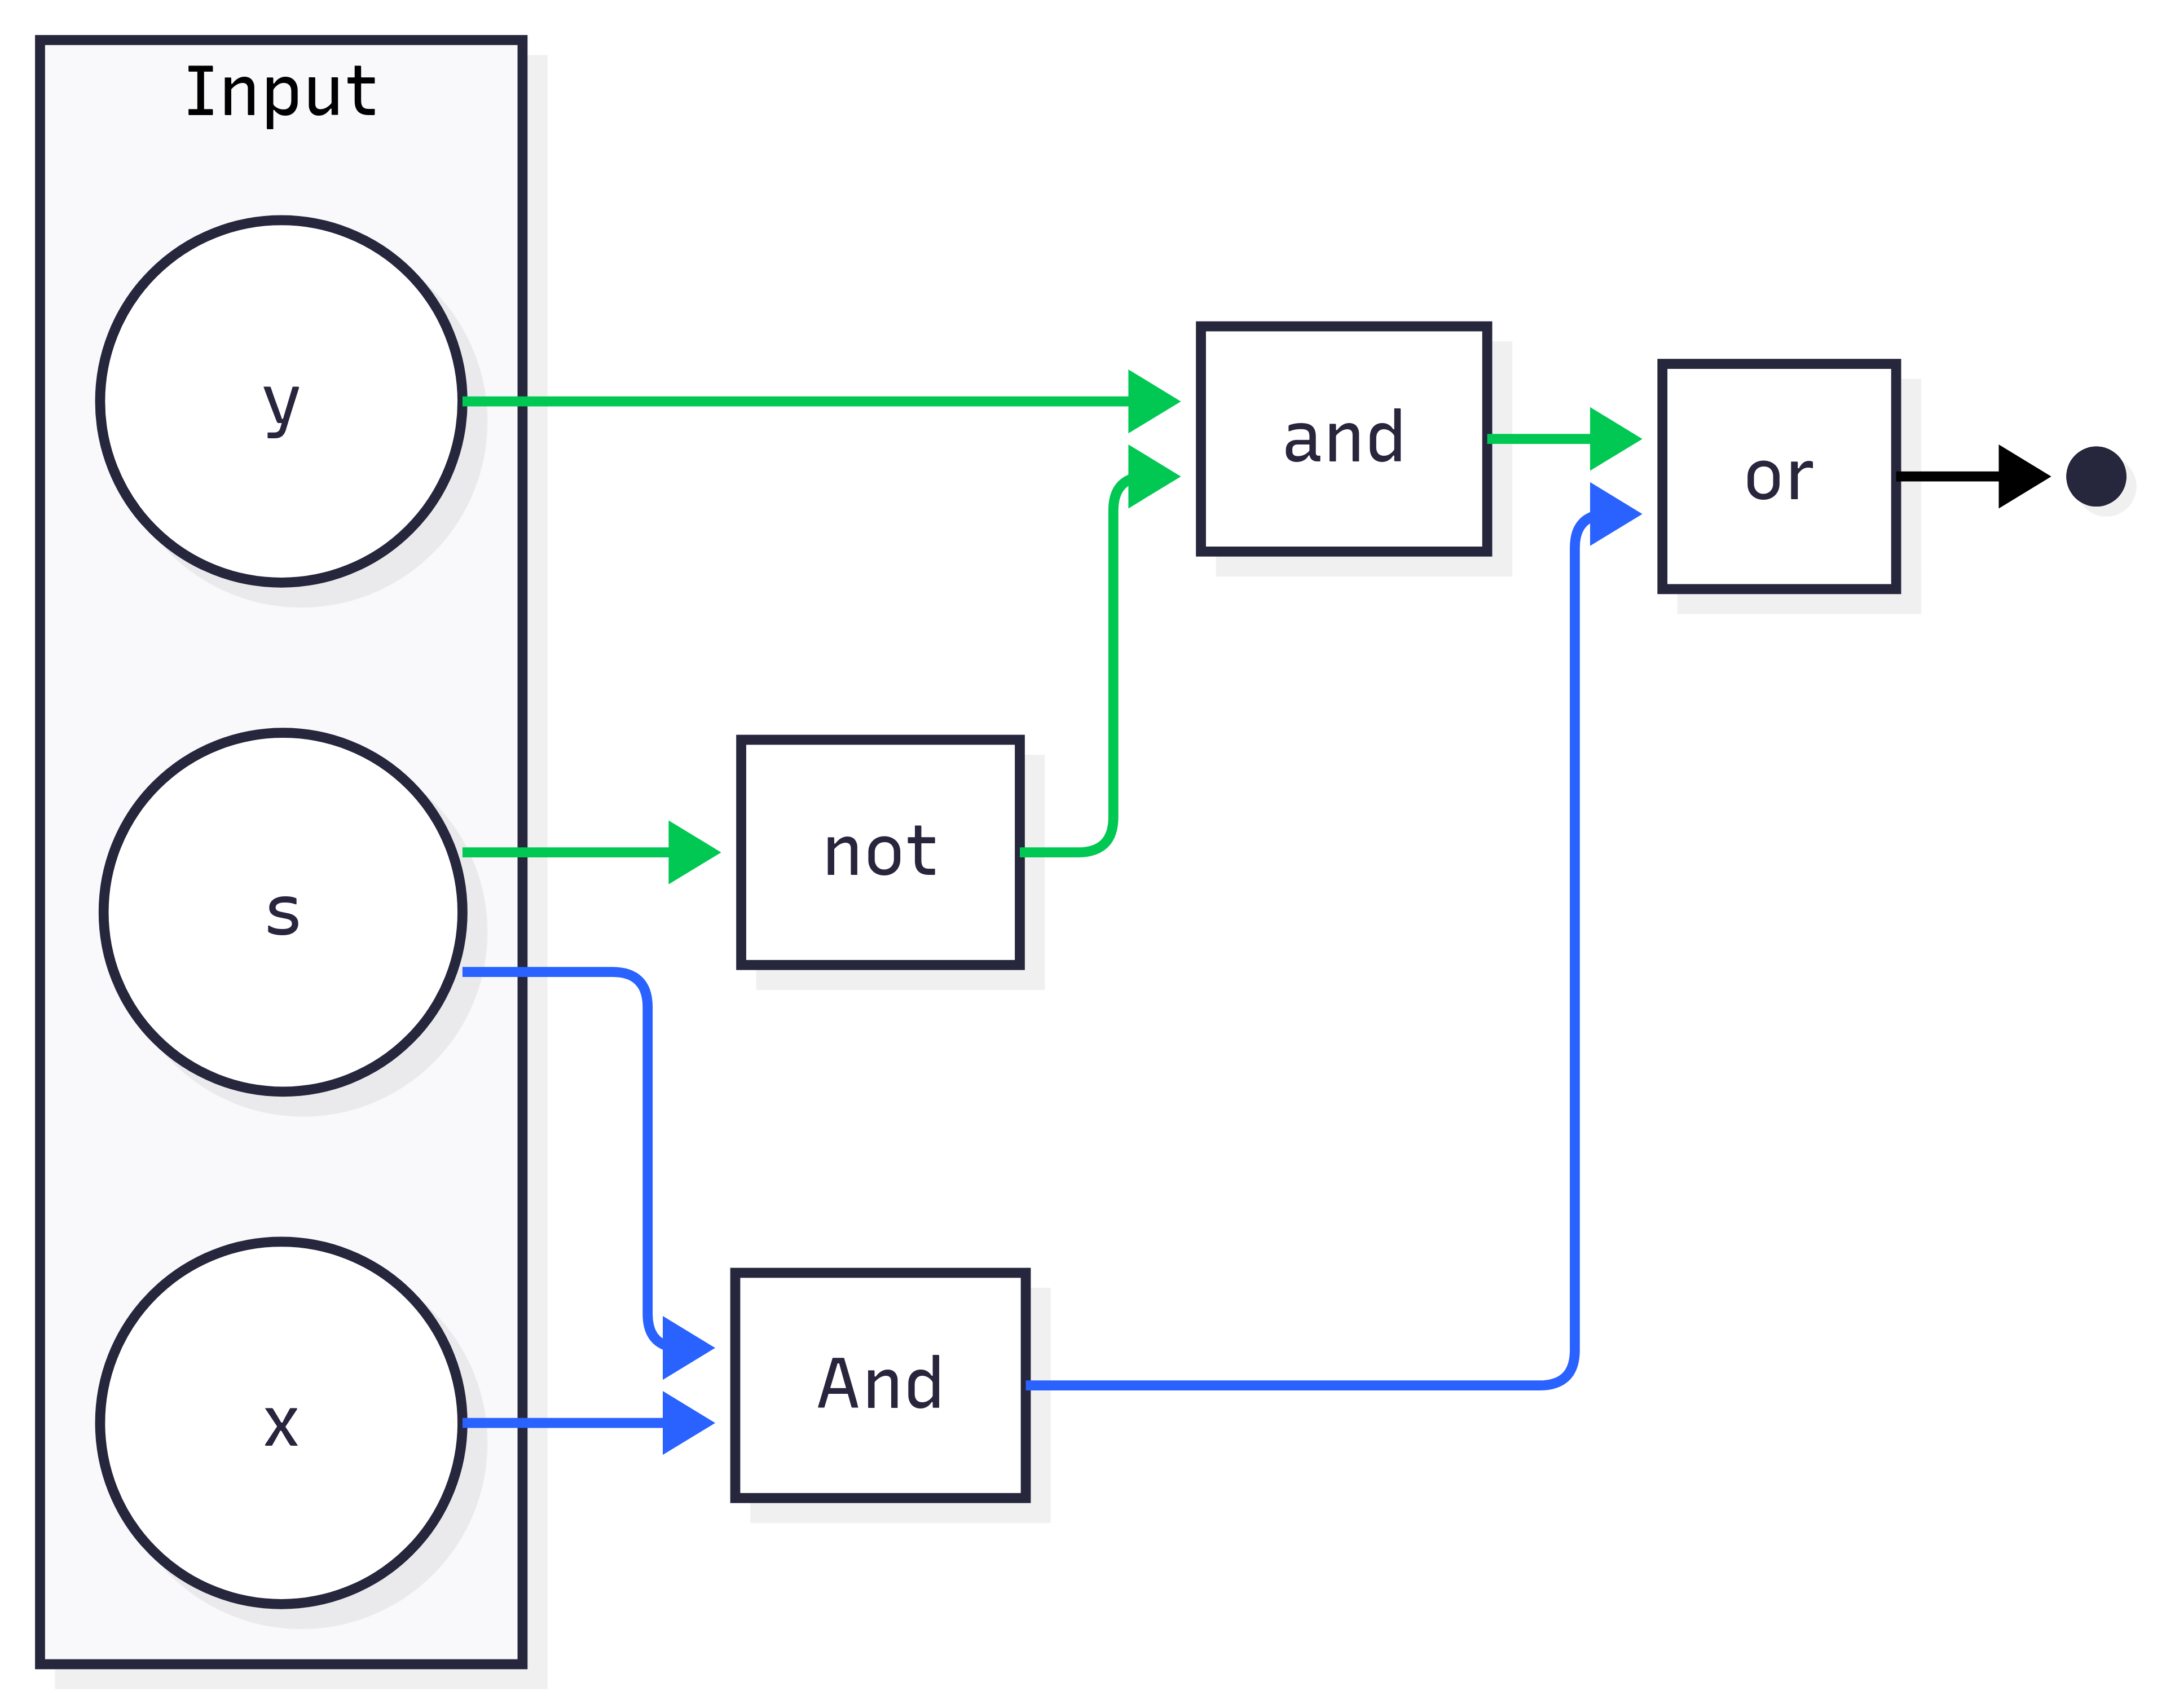
\includegraphics[width=0.3\textwidth]{assets/hazard_circuit.png}}
    \subfloat[Hazard free multiplexer]{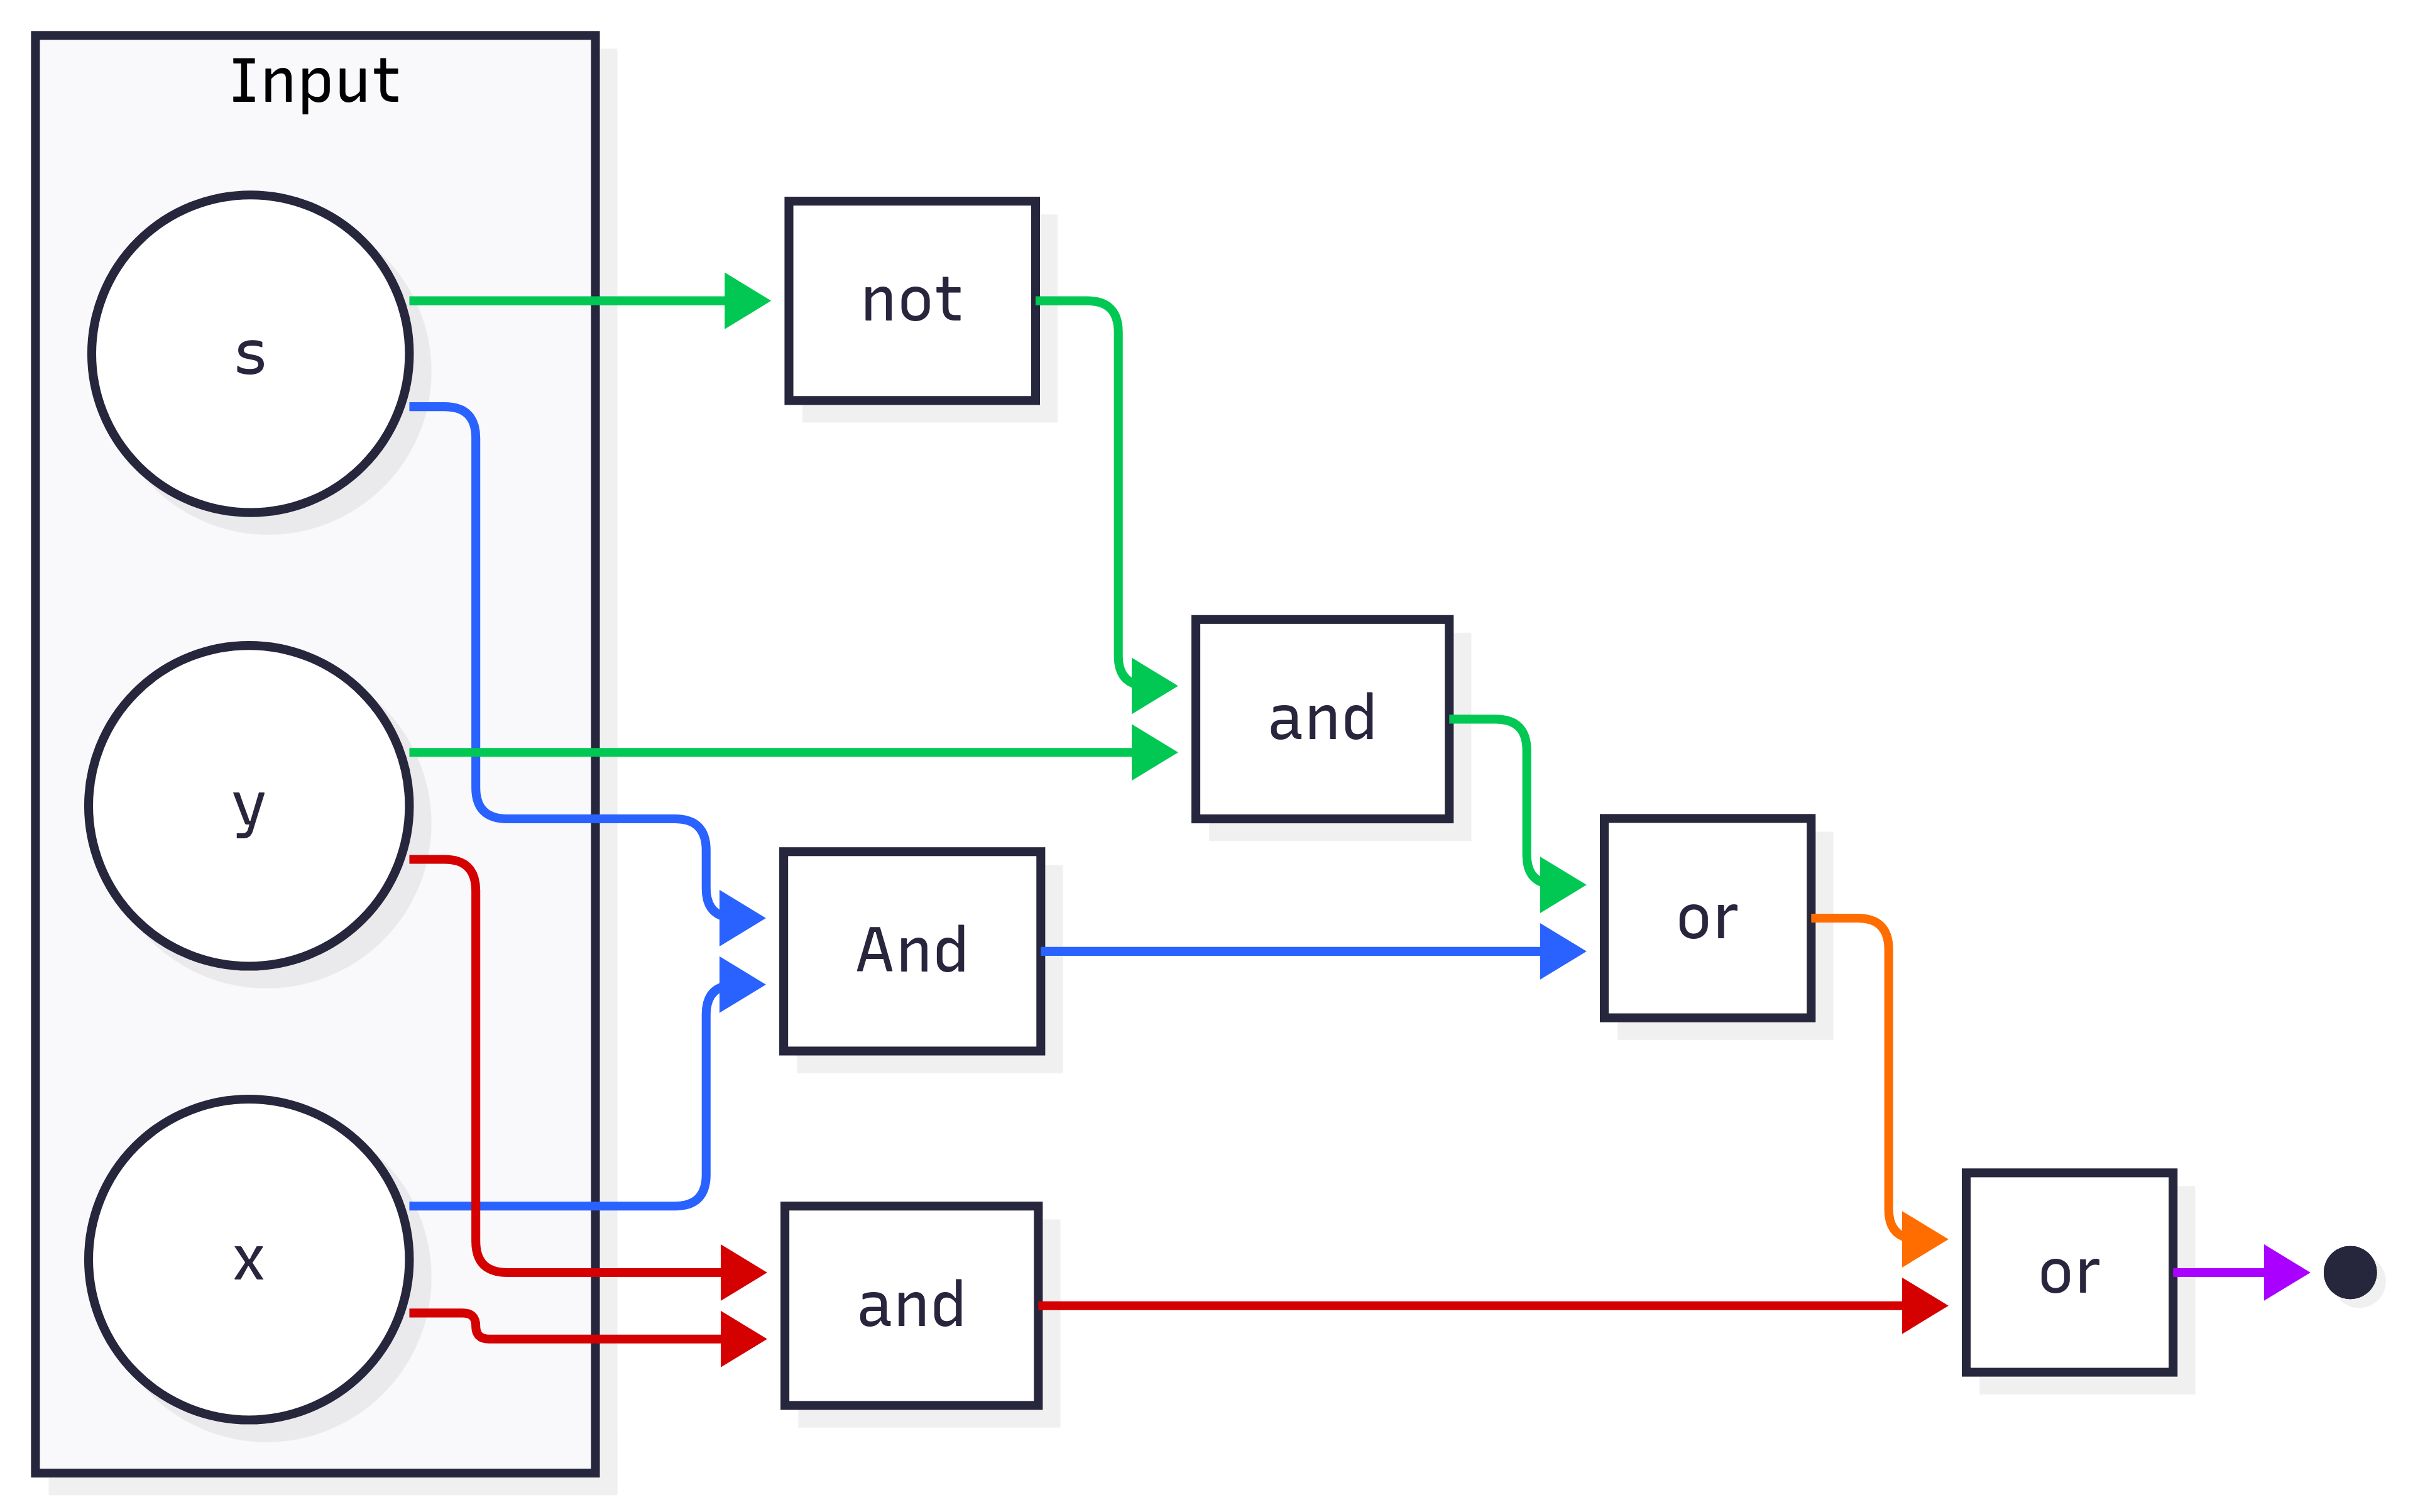
\includegraphics[width=0.3\textwidth]{assets/hazard-free-circuit.png}}
    \caption{Hazard circuit and hazard-free circuit. Figure by \cite{ikenmeyer_ComplexityHazardfreeCircuits_2019}}\label{fig:hazard-example}
\end{figure}

\begin{definition}[K-bit Hazard]
    For $k \in \mathbb{N}$ at $x \in \mathbb{T}^n \iff C$  has a \textit{hazard} at $x$ and $\bot$ appears at most $k$ times in $x$
\end{definition}
%
%
%
